\documentclass[border=6pt]{standalone}
\usepackage{tikz}
\usepackage[edges]{forest}
\usetikzlibrary{arrows.meta,positioning,calc,decorations.pathreplacing,shapes.geometric}
\begin{document}
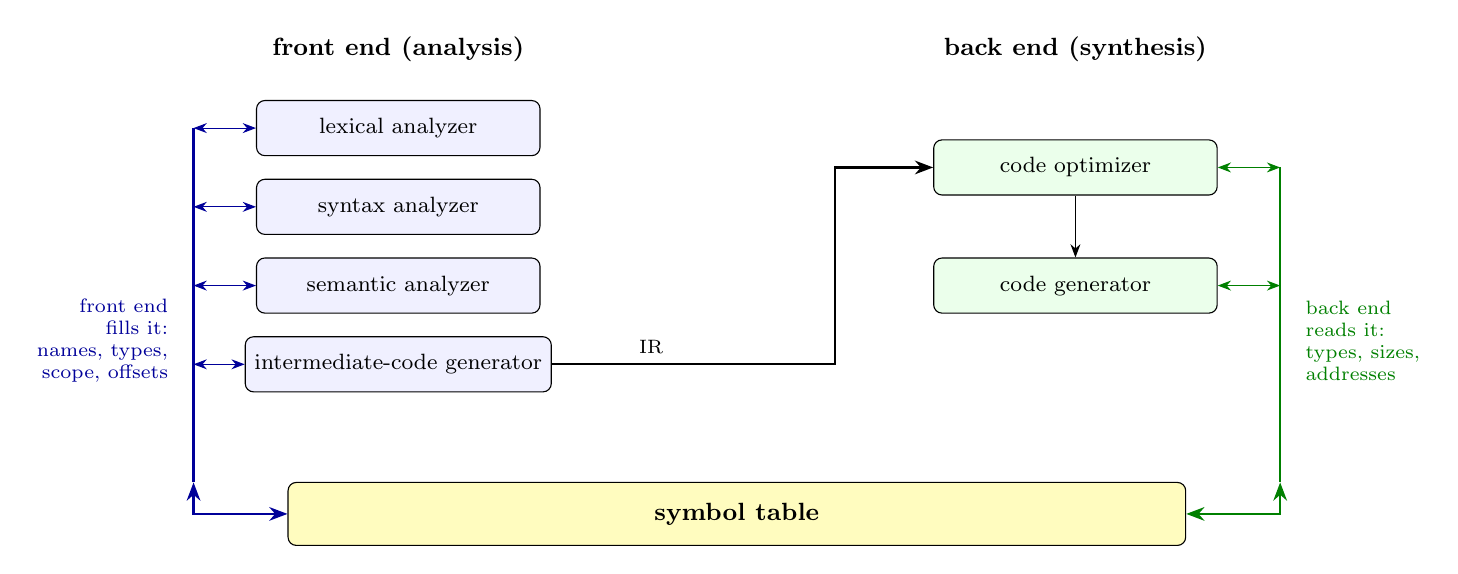
\begin{tikzpicture}[>=Stealth,font=\small,
 ph/.style={draw,rounded corners=3pt,fill=blue!6,minimum width=3.6cm,minimum height=0.7cm,align=center,font=\footnotesize},
 bph/.style={draw,rounded corners=3pt,fill=green!8,minimum width=3.6cm,minimum height=0.7cm,align=center,font=\footnotesize}]
\node[font=\small\bfseries] at (0,4.7) {front end (analysis)};
\node[font=\small\bfseries] at (8.6,4.7) {back end (synthesis)};
\node[ph] (lx) at (0,3.7) {lexical analyzer};
\node[ph] (sx) at (0,2.7) {syntax analyzer};
\node[ph] (sm) at (0,1.7) {semantic analyzer};
\node[ph] (ic) at (0,0.7) {intermediate-code generator};
\node[bph] (op) at (8.6,3.2) {code optimizer};
\node[bph] (cg) at (8.6,1.7) {code generator};
\draw[->,thick] (ic.east) -- node[above,font=\scriptsize,pos=0.35]{IR} ++(3.6,0) |- (op.west);
\draw[->] (op) -- (cg);
\node[draw,rounded corners=3pt,fill=yellow!25,minimum width=11.4cm,minimum height=0.8cm,align=center] (st) at (4.3,-1.2) {\textbf{symbol table}};
% bus on the left for the front end, on the right for the back end
\draw[thick,blue!60!black] (-2.6,-0.8) -- (-2.6,3.7);
\foreach \p/\y in {lx/3.7,sx/2.7,sm/1.7,ic/0.7} \draw[<->,blue!60!black] (\p.west) -- (-2.6,\y);
\draw[<->,thick,blue!60!black] (-2.6,-0.8) -- (-2.6,-1.2) -- (st.west);
\draw[thick,green!50!black] (11.2,-0.8) -- (11.2,3.2);
\foreach \p/\y in {op/3.2,cg/1.7} \draw[<->,green!50!black] (\p.east) -- (11.2,\y);
\draw[<->,thick,green!50!black] (11.2,-0.8) -- (11.2,-1.2) -- (st.east);
\node[font=\scriptsize,anchor=east,align=right,blue!60!black] at (-2.8,1.0) {front end\\fills it:\\names, types,\\scope, offsets};
\node[font=\scriptsize,anchor=west,align=left,green!50!black] at (11.4,1.0) {back end\\reads it:\\types, sizes,\\addresses};
\end{tikzpicture}
\end{document}
